% !TEX encoding = IsoLatin
%\documentclass[twoside]{article}
\documentclass{article}
\usepackage[francais]{babel}
\usepackage[utf8]{inputenc} 
\usepackage[T1]{fontenc}

\usepackage{amsmath}
\usepackage{amssymb}
\usepackage{amsfonts}
\usepackage{graphicx}
\usepackage{bbm}
\usepackage{diagbox}

\usepackage[hmarginratio=1:1,top=32mm,columnsep=20pt]{geometry}
\usepackage{multirow}
\usepackage{multicol} % Style double colonne 
\usepackage{abstract} % Customization de l'abstract 
\usepackage{fancyhdr} % en-têtes et pieds de page 
\usepackage{float} % Nécessaire pour les tables et figures dans l'environnement double colonne 

\usepackage{capt-of}

\usepackage[justification=centering]{caption} % Centré les captions des figures

\usepackage[colorlinks=true,linkcolor=red,urlcolor=blue,filecolor=green]{hyperref} % hyperliens 

% \usepackage{dtklogos}

% En-têtes et pieds de page 
\pagestyle{fancy}  
\fancyhead{} % Blank out the default header
\fancyfoot{} % Blank out the default footer
\fancyhead[C]{Compte rendu TP 3 SY09} % Custom header text
\fancyfoot[RO, LE]{\thepage} % Custom footer text

%\setlength{\parskip}{1ex} % espace entre paragraphes 

\newcommand{\bsx}{\boldsymbol{x}}
\newcommand{\transp}{^{\mathrm{t}}}

\usepackage{color}
\usepackage{listings}
\lstset{
language=R,
basicstyle=\scriptsize\ttfamily,
commentstyle=\ttfamily\color{blue},
numbers=left,
numberstyle=\ttfamily\color{black}\footnotesize,
stepnumber=1,
numbersep=5pt,
backgroundcolor=\color{white},
showspaces=false,
showstringspaces=false,
showtabs=false,
frame=single,
tabsize=2,
captionpos=b,
breaklines=true,
breakatwhitespace=false,
title=\lstname,
escapeinside={},
keywordstyle={},
morekeywords={}
}

%----------------------------------------------------------------------------------------

\title{Compte rendu TP 3 SY09}

\author{ARTCHOUNIN Daniel / VALLOIS Célestin}
\date{\today}

%----------------------------------------------------------------------------------------

\begin{document}

\maketitle % Insert title

\thispagestyle{fancy} % All pages have headers and footers


%----------------------------------------------------------------------------------------

\begin{abstract}

Dans le cadre du troisième sujet des séances de Travaux Pratiques (TP) de l'Unité de Valeur (UV) SY09 enseignée à l'Université de Technologie de Compiègne (UTC), nous avons principalement effectué des classifications et appliqué la théorie bayésienne de la décision sur plusieurs jeux de données binaires.

Dans un premier temps, nous avons implémenté, testé et étudié les performances du \texttt{classifieur euclidien} et des \texttt{$K$ plus proches voisins} sur les cinq jeux de données binaires : \texttt{Synth1-40}, \texttt{Synth1-100}, \texttt{Synth1-500}, \texttt{Synth1-1000} et \texttt{Synth2-1000}.

Dans un second temps, nous avons appliqué la théorie bayésienne sur ces mêmes données.

Le dossier \texttt{code\_source} associé au présent rapport et contenant le code source \texttt{R} écrit afin de répondre aux différentes questions présentes dans le sujet s'organise ainsi : 

\begin{itemize}
  \item \texttt{ex1\_1\_1.R} : le script \texttt{R} associé à la sous sous section \ref{subsubsec_classifieur_euclidien}
  \item \texttt{ex1\_1\_2.R} : le script \texttt{R} associé à la sous sous section \ref{subsubsec_k_plus_proches_voisins}
  \item \texttt{ex1\_1\_3.R} :  le script \texttt{R} associé à la sous section \ref{subsec_programmation}
  \item \texttt{ex1\_2\_1.R} : le script \texttt{R} associé à la sous sous section \ref{subsubsec_dataset_1}
  \item \texttt{ex1\_2\_2.R} :  le script \texttt{R} associé à la sous sous section \ref{subsubsec_dataset_2}
  \item \texttt{ex2.R} : le script \texttt{R} associé à la section \ref{sec_regle_bayes}
\end{itemize}

\end{abstract}

%----------------------------------------------------------------------------------------

\begin{multicols}{2} % Style double colonne 

\section{Classifieur euclidien, $K$ plus proches voisins}
\label{sec_classifieur_euclidien}

\subsection{Programmation}
\label{subsec_programmation}

\subsubsection{Classifieur euclidien}
\label{subsubsec_classifieur_euclidien}

Dans un premier temps, nous avons programmé la fonction \texttt{ceuc.app} d'apprentissage des paramètres du classifieur euclidien et la fonction \texttt{ceuc.val} de classement d'un tableau d'individus-variables avec ce classifieur. La combinaison de ces deux fonctions nous permet d'obtenir un vecteur d'étiquettes prédites pour le tableau individus-variables \texttt{Xtst} transmis en paramètre de la deuxième fonction. Afin de tester ces dernières, nous avons sélectionné certains des individus et des étiquettes du jeu de données \texttt{Synth1-40} de manière à former un ensemble d'apprentissage de $27$ individus et un ensemble de test de $10$  individus. Ensuite, nous avons affiché la frontière de décision associée à l'aide des fonctions précédemment présentées et de la fonction \texttt{front.ceuc}. Nous obtenons le résultat présent dans la figure \ref{fig_decision_boundary_40_test_euclidien}. Comme prévu, la frontière de décision semble être la médiatrice du segment formée par les centres de gravité des deux classes.

\begingroup
   \centering
   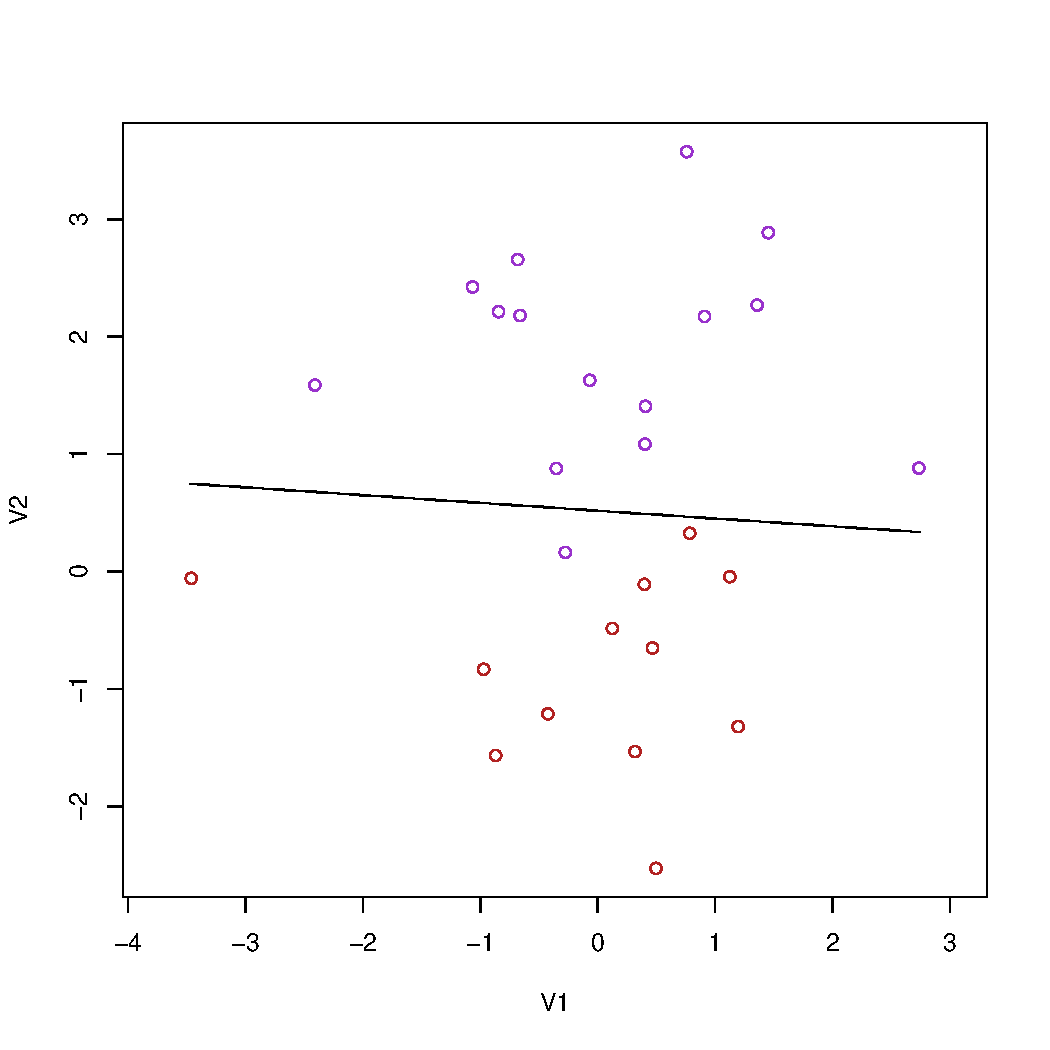
\includegraphics[width=0.35\textwidth]{test_classifieur_euclidien.pdf}
    \captionof{figure}{Frontière de décision pour le jeu de données \texttt{Synth1-40} afin de tester le classifieur euclidien} \label{fig_decision_boundary_40_test_euclidien}
\endgroup

\subsubsection{$K$ plus proches voisins}
\label{subsubsec_k_plus_proches_voisins}

Pour les $K$ plus proches voisins, nous avons programmé une fonction \texttt{kppv.tune} déterminant le nombre "optimal" de voisins $K_{opt}$ et la fonction \texttt{kppv.val} de classement d'un tableau d'individus-variables. La combinaison de ces deux fonctions nous permet d'obtenir un vecteur d'étiquettes prédites correspondant au tableau individus-variables \texttt{Xtst} transmis en paramètre de la deuxième fonction. A nouveau, afin de tester nos deux fonctions, nous avons sélectionné certains des individus et des étiquettes du jeu de données \texttt{Synth1-40} de manière à former un ensemble d'apprentissage de $18$ individus, un ensemble de validation de $9$ individus et un ensemble de test de $10$ individus. Pour ce jeu de données, la difficulté dans l'écriture de la fonction \texttt{kppv.tune} était la présence de plusieurs $K$ présentant le même taux d'erreur. Afin d'y faire face, nous avons décidé de sélectionner le plus grand $K$ minimisant le taux d'erreur afin d'être le moins "naïf" possible sur l'ensemble de validation envoyé en paramètre de la fonction (afin que le modèle puisse plus facilement s'adapter à d'autres jeux de données). Cette décision n'aura évidemment pas un impact important sur la suite de notre rapport : ce cas ne se présente généralement pas lorsque l'on manipule des jeux de données "plus" volumineux. 

La frontière de décision obtenue avec le jeu de données \texttt{Synth1-40} est consultable dans la figure \ref{fig_decision_boundary_40_test_kppv}. On notera, que pour ce jeu de données, $K_{opt} = 5$.

\begingroup
   \centering
   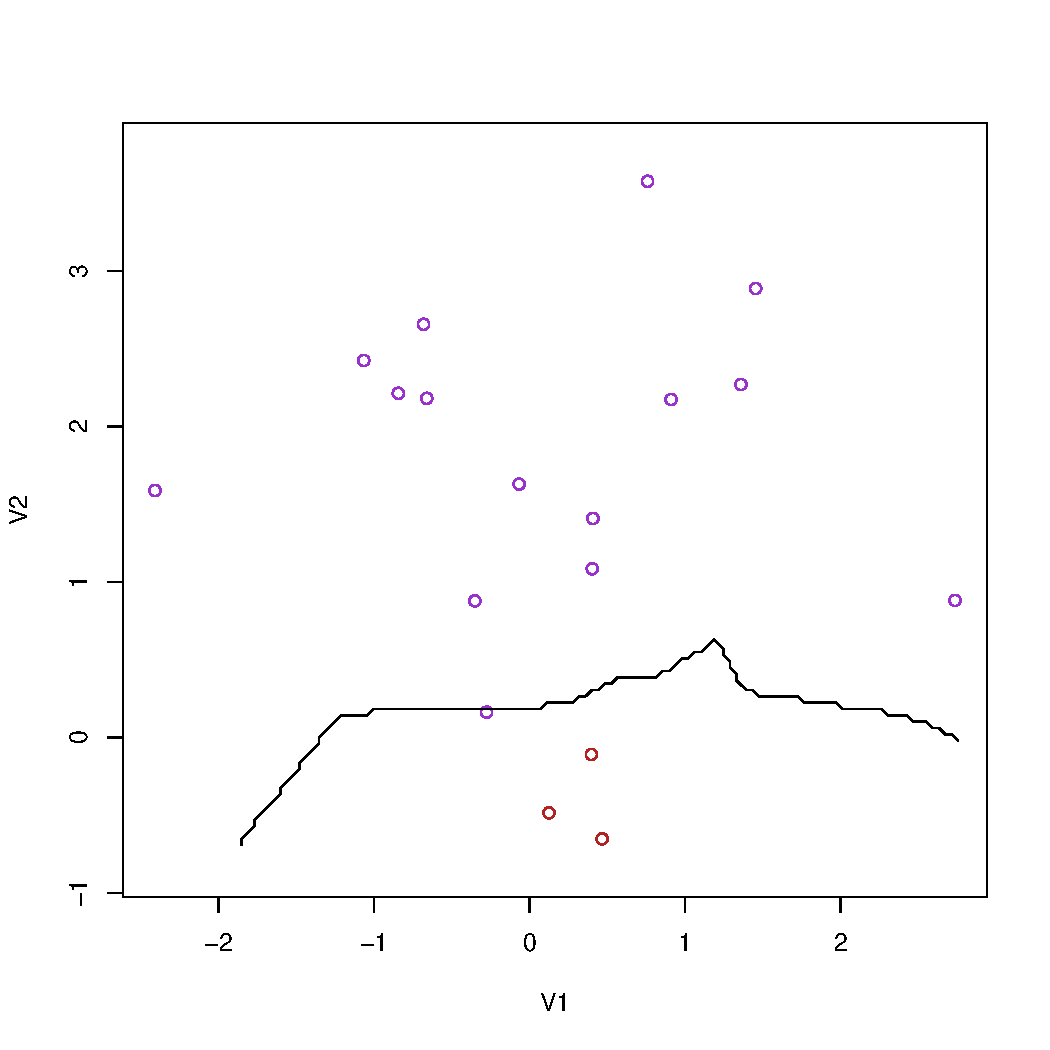
\includegraphics[width=0.35\textwidth]{test_k_plus_proches_voisins.pdf}
    \captionof{figure}{Frontière de décision pour le jeu de données \texttt{Synth1-40} afin de tester les $K$ plus proches voisins}
    \label{fig_decision_boundary_40_test_kppv}
\endgroup

\subsection{Évaluation des performances}
\label{subsec_evaluation_performances}

\subsubsection{Jeux de données Synth1-40, Synth1-100, Synth1-500 et Synth1-1000}
\label{subsubsec_dataset_1}

Dans un premier temps, nous avons estimé les paramètres $\mu_k$ et $\Sigma_k$ des distributions conditionnelles, ainsi que les proportions $\pi_k$ des classes.

Soit une population $\mathcal{P}$ d'individus $X_i, i=1 \cdots n$, où chacun est décrit par $p$ variables (dans notre cas, $p=2$). Soit un vecteur $Z$ de taille $n$ décrivant la classe de chaque individu. Soit $\pi_k$ la proportion de la classe $k, k \in \{1; \cdots; g \}$ (dans notre cas $g = 2$). L'énoncé mentionne également que, conditionnellement à son appartenance à la classe $k$, $X_i \sim \mathcal{N}(\mu_k, \Sigma_k).$ 

Définissons $t_{ik}$ ainsi :
\[
t_{ik} = 
\left\{ 
\begin{array}{l}
1, \text{\ si \ } z_i = w_k \\
0, \text{\ sinon.} 
\end{array}
\right.
\]

En posant $n_k$ le nombre d'individus dans la classe $k, k \in \{1; 2 \}$, les estimateurs des paramètres $\pi_k, \mu_k$ et $\Sigma_k$ sont $\widehat{\pi}_k, \widehat{\mu}_k$ et $\widehat{\Sigma}_k$, où
\[
\widehat{\pi}_k = \frac{n_k}{n}, \widehat{\mu}_k = \bar{X}
\]
et
\[
\widehat{\Sigma}_k = \frac{1}{n} \sum_i^{n}(X_i - \widehat{\mu}_k)(X - \widehat{\mu}_k)^T .
\]

Voici les résultats obtenus pour nos $4$ jeux de données \texttt{Synth1}.

\begin{center}
{\footnotesize
\begin{tabular}{|@{}c@{}|@{}c@{}||@{}c@{}|@{}c@{}|c|}
\hline
\multicolumn{2}{|c|}{\texttt{Synth1-}} & $\widehat{\mu}_k$ & $\widehat{\Sigma}_k$ & $\widehat{\pi}_k$  \\
\hline
\hline
\texttt{40} & $k=1$ & (-0.049  1.976) & $\begin{pmatrix}
    1.386 & -0.104 \\
   -0.104 & 0.855
\end{pmatrix}$
  & 0.575 \\
\cline{2-3}
 & $k=2$  & (0.110 -0.696) & $\begin{pmatrix}
   1.646 & -0.304 \\
  -0.304 & 0.783
\end{pmatrix}$ & 0.425 \\
\hline
\hline
\texttt{100} & $k=1$ & (0.168 2.060) & $\begin{pmatrix}
   0.873 & 0.069 \\
   0.069 & 0.868 
\end{pmatrix}$
  & 0.46 \\
\cline{2-3}
 & $k=2$  & (-0.187 -1.064) & $\begin{pmatrix}
  0.884 & 0.068 \\
  0.068 & 0.601
\end{pmatrix}$ & 0.54 \\
\hline
\hline
\texttt{500} & $k=1$ & (0.028 2.004) & $\begin{pmatrix}
   0.990 & 0.004 \\
   0.004 & 0.940 
\end{pmatrix}$
  & 0.516 \\
\cline{2-3}
 & $k=2$  & (-0.034 -0.901) & $\begin{pmatrix}
   0.895 & -0.023 \\
   -0.023 & 0.813
\end{pmatrix}$ & 0.484 \\
\hline
\hline
\texttt{1000} & $k=1$ & (-0.084  1.985) & $\begin{pmatrix}
   1.028 & 0.054 \\
   0.054 & 1.014
\end{pmatrix}$
  & 0.481 \\
\cline{2-3}
 & $k=2$  & (-0.038 -1.013) & $\begin{pmatrix}
  0.975 & -0.019 \\
  -0.019 & 0.953 
\end{pmatrix}$ & 0.519 \\ 
\hline
\end{tabular}
}
\end{center}

Nous remarquons que plus l'échantillon est grand, plus $\widehat{\mu}_1$ et $\widehat{\mu}_2$ semblent respectivement se rapprocher de $\begin{pmatrix} 0 \\ 2 \end{pmatrix}$ et de $\begin{pmatrix} 0 \\ -1 \end{pmatrix}$
De même, plus l'échantillon est grand, plus $\widehat{\Sigma}_1$  et $\widehat{\Sigma}_2$ semblent tous deux se rapprocher de $\begin{pmatrix}
  1  & 0 \\
  0 & 1  
\end{pmatrix}$. Le constat est identique pour $\widehat{\pi}_1$ et $\widehat{\pi}_2$ qui semblent tous les deux se rapprocher de $0.5$.

Sachant que les estimateurs du maximum de vraisemblance sont des estimateurs convergents, il est très probable que les valeurs réelles de ces paramètres soient proches de celles énoncées ci-dessus. Ainsi, un classifieur euclidien semble particulièrement bien adapté à ces $4$ jeux de données.

Ensuite, nous avons écrit un script qui effectue $N = 20$ séparations aléatoires de chacun des $4$ jeux de données en ensembles d’apprentissage et de test, puis, qui calcule pour chacune leur taux d’erreur d’apprentissage ainsi que leur taux d’erreur de test.

En considérant l’ensemble des résultats obtenus lors des $N = 20$ expériences, nous avons calculé l’estimation ponctuelle $\widehat{\varepsilon} = \bar{\varepsilon}$ du taux d’erreur $\varepsilon$ ainsi qu’un intervalle de confiance bilatéral $IC_\varepsilon$ pour le même paramètre au niveau de confiance $1 - \alpha,$ où $\alpha = 0.05$. 

Pour ce faire, sachant que le phénomène aléatoire $\varepsilon$ auquel on s'intéresse suit une loi que l'on ne connaît pas d'espérance $\mu$ et de variance $\sigma^2$, l'intervalle de confiance bilatéral $IC_\varepsilon$ approché est celui-ci :
\begin{equation}
	\label{eq_confidence_interval}
	IC_\varepsilon = \left[ \widehat{\varepsilon} - u_{1 - \frac{\alpha}{2}} \frac{S^{\ast}}{\sqrt{N}}, \widehat{\varepsilon} + u_{1 - \frac{\alpha}{2}} \frac{S^{\ast}}{\sqrt{N}} \right],
\end{equation}
où $S^{\ast}$ l'écart-type corrigé de $\varepsilon$.

En pratique, cette approximation est utilisée lorsque $N \geq 30.$ Toutefois, ne connaissant pas assez $\varepsilon$, on est contraint d'utiliser $IC_\varepsilon$ bien que cela puisse conduire à des résultats de moins bonne qualité.

Ci-dessous, figurent les estimations faites sur l’ensemble d’apprentissage, puis, celles faites sur l’ensemble de test.

{\footnotesize
\begin{center}
\begin{tabular}{| @{}c@{} || @{}c@{} | c | c |}
\hline
\texttt{Synth1-} & Type d'ensemble & $\widehat{\varepsilon}$  & $IC_\varepsilon$  \\
\hline
\hline
\texttt{40} & Apprentissage & 0.065 & [0.045, 0.086] \\
\cline{2-4}
 & Test & 0.1 & [0.069, 0.131] \\
\hline
\hline
\texttt{100} & Apprentissage & 0.051 & [0.042, 0.060] \\
\cline{2-4}
 & Test & 0.059 & [0.044, 0.074] \\
\hline
\hline
\texttt{500} & Apprentissage & 0.051 & [0.048, 0.054] \\
\cline{2-4}
 & Test & 0.054 & [0.048, 0.059] \\
\hline
\hline
\texttt{1000} & Apprentissage & 0.064 & [0.062, 0.066] \\
\cline{2-4}
 & Test & 0.070 & [0.064, 0.076] \\
\hline
\end{tabular}\\ 
\end{center}
}

Nous observons que, pour les ensembles d'apprentissage, et, pour les ensembles de tests, plus la taille du jeu de données est conséquente, plus la taille d'$IC_\varepsilon$ semble diminuer. Dans notre expérience, nous savons que seul $S^{\ast}$ impacte la taille d'$IC_\varepsilon$ ($\alpha$ et $N$ sont constants). Ainsi, cette tendance traduit une baisse de $S^{\ast}$. Or, $S^{\ast}$ converge en probabilité vers $\sigma$. Ainsi, les résultats obtenus semblent montrer que plus la taille d'un jeu de données est grande, plus la variance de son taux d'erreur est basse.

De plus, on constate que le taux d'erreur d'apprentissage semble moins élevé que le taux d'erreur de test. Ce résultat est tout à fait cohérent puisque le modèle apprend ces paramètres via l'ensemble d'apprentissage. Ainsi, il est logique que les paramètres du modèle soient plus "adaptés" pour l'ensemble d'apprentissage que pour l'ensemble de test. Ce résultat justifie évidemment l'usage d'un ensemble de test. Effectivement, l'estimateur du taux d'erreur d'apprentissage est biaisé en faveur du modèle. 

Par ailleurs, pour les ensembles d'apprentissage et pour les ensembles de tests, la taille du jeu de données ne semble pas avoir d'impact particulier sur le taux d'erreur. 

Ensuite, nous effectuons une séparation aléatoire de l’ensemble des $4$ jeux de données en un ensemble d’apprentissage et un ensemble de test. Nous pouvons alors déterminer le nombre optimal de voisins à l’aide de la fonction \texttt{kppv.tune} que nous avons précédemment codé. Ce calcul se fera en utilisant l’ensemble d’apprentissage comme ensemble de validation. 

Nous obtenons alors un nombre optimal de voisin $K_{opt}$ de valeur $1$. Ce résultat était évidemment prévisible car nous prenons l’ensemble d’apprentissage comme ensemble de validation. Supposons que l'on s'intéresse au cas où $K=1$ voisin, le plus proche est forcément le point lui-même. Par conséquent, la classification est toujours correcte et le taux d’erreur vaut toujours $0$. Ainsi, $K_{opt} = 1$.

A l'instar du travail effectué pour le \textbf{classifieur euclidien}, après avoir effectué $N=20$ séparations aléatoires, nous calculons à nouveau pour chacun des $4$ jeux de données les estimations ponctuelles  $\widehat{\varepsilon} = \bar{\varepsilon}$ du taux d’erreur $\varepsilon$ et les intervalles de confiance $IC_\varepsilon$ sur les ensembles d’apprentissage et de tests de ces derniers. Toutefois, ils sont dorénavant calculées après l'utilisation de l'algorithme des $K$ plus proches voisins (et non après le classifieur euclidien). On pourra également noter que les jeux de données sont dorénavant a priori séparés en $3$ ensembles : un d'apprentissage, un de test et un de validation. Nous précisons que l'intervalle de confiance reste celui définie dans l'équation \ref{eq_confidence_interval} et que les remarques lui étant associées restent valables.

{\footnotesize
\begin{center}
\begin{tabular}{|c||c|c|c|c|}
\hline
\texttt{Synth1-} & Type d'ensemble & $\widehat{\varepsilon}$  & $IC_\varepsilon$  \\
\hline
\hline
\texttt{40} & Apprentissage & 0.065 & [0.044,  0.086] \\
\cline{2-4}
 & Test & 0.125 & [0.085, 0.165] \\
\hline
\hline
\texttt{100} & Apprentissage &  0.054 & [0.040, 0.068] \\
\cline{2-4}
 & Test & 0.069 & [0.045, 0.093] \\
\hline
\hline
\texttt{500} & Apprentissage & 0.052 & [0.047, 0.057] \\
\cline{2-4}
 & Test & 0.058 & [0.049, 0.067] \\
\hline
\hline
\texttt{1000} & Apprentissage & 0.059 & [0.055, 0.063] \\
\cline{2-4}
 & Test & 0.072 & [0.065, 0.079] \\
\hline
\end{tabular}
\end{center}
}

A nouveau, nous observons que, pour les ensembles d'apprentissage, et, pour les ensembles de tests, plus la taille du jeu de données est conséquente, plus la taille d'$IC_\varepsilon$ semble diminuer. Ainsi, à nouveau les résultats obtenus semblent montrer que plus la taille d'un jeu de données est grande, plus la variance de son taux d'erreur est basse. 

De même, on constate à nouveau que le taux d'erreur d'apprentissage est moins élevé que le taux d'erreur de test.

De plus, pour les ensembles d'apprentissage et pour les ensembles de tests, la taille du jeu de données ne semble pas avoir d'impact particulier sur le taux d'erreur. 

Après comparaison avec les résultats obtenus via le classifieur euclidien, nous constatons que, pour tous les jeux de données, $\varepsilon_{tst_{ppv}} > \varepsilon_{tst_{ceuc}}.$ Ce résultat est à nouveau cohérent. Effectivement, nous savons que les lois conditionnelles des individus des deux classes des lois normales bivariées ainsi que $\Sigma_1 \approx I_2$, $\Sigma_2 \approx I_2$ et $\Sigma_1 \approx \Sigma_2.$ Ainsi, intuitivement, nous savons que la médiatrice du segment formé par les centres des deux classes serait une "bonne" frontière de décision. Or, il s'avère qu'il s'agit de la frontière de décision du classifieur euclidien. De plus, l'algorithme des $K$ plus proches voisins semble plus adapté à des cas où les frontières de décision sont plus complexes. Ainsi, cela explique les résultats obtenus. 

En observant d'une manière plus approfondie, nous pouvons constater l'inégalité suivante :
\[
|\varepsilon_{app_{ppv}} - \varepsilon_{tst_{ppv}}| > |\varepsilon_{app_{ceuc}} - \varepsilon_{tst_{ceuc}}|.
\]

Toutefois, la différence entre les deux ensembles étant très mince, nous ne pouvons pas tirer de conclusion intéressante de cette remarque.

Pour le classifieur de distances euclidiennes, les résultats des deux ensembles sont assez similaires. Cependant, pour le classifieur des $K$ plus proches voisins, les résultats de l’ensemble d’apprentissage semblent plus faibles que ceux de l’ensemble de test. 

\subsubsection{Jeux de données Synth2-1000}
\label{subsubsec_dataset_2}

Nous utilisons la même méthode pour le calcul des estimateurs $\widehat{\pi}_k, \widehat{\mu}_k$ et $\widehat{\Sigma}_k$ des paramètres $\pi_k, \mu_k$ et $\Sigma_k$.

\begin{center}
{\footnotesize
\begin{tabular}{|@{}c@{}|c||@{}c@{}|@{}c@{}|c|}
\hline
\multicolumn{2}{|c|}{Synth2} & $\widehat{\mu}_k$ & $\widehat{\Sigma_k}$ & $ \widehat{\pi}_k$  \\
\hline
\hline
1000 & $ k=1 $ & (-0.072 2.945) & $\begin{pmatrix}
  1.067 & -0.053 \\
  -0.053 & 1.067 
\end{pmatrix}$
  & 0.486 \\
\cline{2-3}
 & $ k=2 $  & (-0.098 -5.101) & $\begin{pmatrix}
  5.207 & 0.114 \\
  0.114 & 5.159 
\end{pmatrix}$ & 0.514 \\
\hline
\end{tabular}
}
\end{center}

Nous remarquons que $\widehat{\mu}_1$ et $\widehat{\mu}_2$ sont respectivement proches de  $\begin{pmatrix} 0 \\ 3 \end{pmatrix}$ et de $\begin{pmatrix} 0 \\ -5 \end{pmatrix}$. \\
De même, $\widehat{\Sigma}_1$ et $\widehat{\Sigma}_2$ sont proches de 
$\begin{pmatrix}
  1 & 0 \\
  0 & 1  
\end{pmatrix}$ et $\begin{pmatrix}
  5 & 0 \\
  0 & 5  
\end{pmatrix}$ 

De plus, $\widehat{\pi}_1$ et $\widehat{\pi}_2$ sont tous deux proches de  $0.5$.

Sachant qu'apparemment $\Sigma_1 \neq \Sigma_2,$ une analyse discriminante linéaire et surtout un classifieur euclidien seraient inadaptés. Cependant, étant donné que l'on possède un jeu de données avec $1000$ individus, on peut penser qu'une analyse discriminante quadratique serait plus adaptée.  

Comme précédemment, nous estimons les résultats avec les deux classifieurs.

Pour le \textbf{classifieur euclidien}, nous obtenons les résultats suivants :

{\footnotesize
\begin{center}
\begin{tabular}{|c||c|c|c|c|}
\hline
Type d'ensemble & $\widehat{\varepsilon}$  & $IC_\varepsilon$  \\
\hline
\hline
Apprentissage & 0.022 & [0.020, 0.023] \\
\hline
Test & 0.022 & [0.019, 0.025] \\
\hline
\end{tabular}
\end{center}
}

Pour les \textbf{$K$ plus proches voisins}, nous obtenons les résultats suivants :

{\footnotesize
\begin{center}
\begin{tabular}{|c||c|c|c|c|}
\hline
Type d'ensemble & $\widehat{\varepsilon}$  & $IC_\varepsilon$  \\
\hline
\hline
Apprentissage & 0.0063 & [0.0044, 0.0081] \\
\hline
Test & 0.0088 & [0.0063, 0.0113] \\
\hline
\end{tabular}
\end{center}
}

Nous obtenons une estimation du taux d'erreur $\widehat{\varepsilon}$ beaucoup plus faible pour les $K$ plus proches voisins que pour le classifieur euclidien. Cela est évidemment cohérent. Effectivement, sachant qu'il y a de fortes chances que $\Sigma_1 \neq \Sigma_2,$ intuitivement, on sait que la médiatrice du segment formé des centres des deux classes ne peut pas être une bonne frontière de décision. Pour ce type de cas, un conique comme frontière de décision semble nettement plus adaptée. Par ailleurs, vu que l'équation de la frontière de décision semble être plus complexe, l'algorithme des $K$ plus proches voisins semble plus adapté. Ainsi, cela justifie les résultats observés.
\section{Règle de Bayes}
\label{sec_regle_bayes}

Les jeux de données étudiés précédemment ont tous été obtenus ainsi :

\begin{enumerate}
	\item tout d'abord, l'effectif $n_1$ de la classe $\omega_1$ a été déterminé par tirage aléatoire suivant une loi binomiale de paramètres $n$ et $\pi_1 = 0.5$
	\item ensuite, $n_1$ individus ont été générés dans la classe $\omega_1$ suivant une loi normale bivariée de paramètres $\mu_1$ et $\Sigma_1$, et $n_2 = n - n_1$ individus ont été générés dans la classe $\omega_2$ suivant une loi normale bivariée de paramètres $\mu_2$ et $\Sigma_2$.
\end{enumerate}

Pour chacun des cinq jeux de données, les paramètres ont la forme suivante
 \begin{equation}
 \label{eq_normale_bivariee}
 	\mu_i = 
	\begin{pmatrix}
	\mu_{i1} \\
	\mu_{i2}
	\end{pmatrix},
	\Sigma_i = 
	\begin{pmatrix}
	\sigma_{11}^2 = \sigma^2 & \sigma_{12}^2 = 0 \\
	\sigma_{21}^2 = 0 & \sigma_{22}^2 = \sigma^2
	\end{pmatrix}, 
\end{equation}
où $i \in \{1 ; 2 \} .$

Soit $X = {(X^1, X^2)}^{T}$ suivant, conditionnellement à la classe $\omega_i$, une loi normale bivariée de paramètres $\mu_i$ et $\Sigma_i, i \in \{1 ; 2 \}, \mu_i$ et $\Sigma_i$ définis selon l'équation $\ref{eq_normale_bivariee}$. Soit $x = {(x_1, x_2)}^{T}$ une réalisation de $X$, on constate que :
\[
f(X^1 = x_1, X^2 = x_2 | \omega_i )
\]

\[
= \frac{1}{2 \pi \sqrt{|\Sigma_i|}} \exp \left(-\frac{1}{2}(x - \mu_i)^T \Sigma_i^{-1} (x - \mu_i) \right) 
\]

\[
\begin{split}
= \frac{1}{2 \pi |\sigma_{11} * \sigma_{22}|} \exp \left( -\frac{1}{2} (x_1 - \mu_{i1}, x_2 - \mu_{i2}) \right. \\
\left. 
\begin{pmatrix}
	\frac{1}{\sigma_{11}^2} & 0 \\
	0 & \frac{1}{\sigma_{22}^2}
\end{pmatrix}
(x_1 - \mu_{i1}, x_2 - \mu_{i2})^T \right)
\end{split}
\]

\[
\begin{split}
= \frac{1}{2\pi \sigma_{11} * \sigma_{22}} \exp \left( -\frac{1}{2} \left( \frac{(x_1 - \mu_{i1})^2}{\sigma_{11}^2} + \right. \right. \\ 
\left. \left. \frac{(x_2 - \mu_{i2})^2}{\sigma_{22}^2} \right) \right)
\end{split}
\]

\[
\begin{split}
= \frac{1}{\sqrt{2 \pi \sigma_{11}^2}} \exp \left( -\frac{1}{2} \left( \frac{(x_1 - \mu_{i1})^2}{\sigma_{11}^2} \right) \right) * \\
\frac{1}{\sqrt{2 \pi \sigma_{22}^2}} \exp \left( -\frac{1}{2} \left( \frac{(x_2 - \mu_{i2})^2}{\sigma_{22}^2} \right) \right)
\end{split}
\]

\[
= f_1(X^1 = x_1) * f_2 (X^2 = x_2)
\]

Autrement dit, $X^1$ et $X^2$ sont indépendantes, $X^1 \sim \mathcal{N}( \mu_{i1}, \sigma_{11}^2 )$ et $X^2 \sim \mathcal{N}( \mu_{i2}, \sigma_{22}^2 )$.


Pour chaque classe $\omega_i, i \in \{1 ; 2 \},$ des cinq jeux de données dont les paramètres ont la forme définie dans l'équation \ref{eq_normale_bivariee}, tentons de prouver que les courbes d'iso-densité sont des cercles dont on calculera les centres et les rayons. Ce problème se ramène donc à résoudre l'équation suivante :
\[
f(X^1 = x_1, X^2 = x_2 | \omega_i) = c
\]

\[
\begin{split}
\implies \frac{1}{2\pi \sigma_{11} * \sigma_{22}} \exp \left( -\frac{1}{2} \left( \frac{(x_1 - \mu_{i1})^2}{\sigma_{11}^2} + \right. \right. 
\\ \left. \left. \frac{(x_2 - \mu_{i2})^2}{\sigma_{22}^2} \right) \right)
= c
\end{split}
\]

\[
\implies \frac{(x_1 - \mu_{i1})^2}{\sigma_{11}^2} + \frac{(x_2 - \mu_{i2})^2}{\sigma_{22}^2} = T
\]

\begin{equation}
\label{eq_ellipse_cartesian}
\implies \frac{(x_1 - \mu_{i1})^2}{\sigma_{11}^2 \sqrt{T}^2} + \frac{(x_2 - \mu_{i2})^2}{\sigma_{22}^2 \sqrt{T}^2} = 1,
\end{equation}
où $T = -2 \ln(2\pi c \sigma_{11} * \sigma_{12}), c \in \mathbb{R}_+^{\star}$ et $c$ choisi tel que $T > 0$.

On constate que l'équation \ref{eq_ellipse_cartesian} est l'équation cartésienne d'une ellipse dans un plan. Cette dernière peut se mettre assez simplement sous la forme paramétrique :

\begin{equation}
  \label{eq_ellipse_parametrique}
  \left\{
    \begin{array}{rcl}
    	x_1 & = & \mu_{i1} + \sigma_{11} \sqrt{T} * \cos(\theta)\\ 
        x_2 & = & \mu_{i2} + \sigma_{22} \sqrt{T} * \sin(\theta)
    \end{array},
  \right.\theta \in [0, 2 \pi[
\end{equation}

Étant donné que dans les cinq jeux de données, $\sigma = \sigma_{11} = \sigma_{22},$ on retrouve le résultat prévu : les courbes d'iso-valeurs sont des cercles de centres $\mu_i = (\mu_{i1}, \mu_{i2})^T $ et de rayons $R = \sigma \sqrt{T}$.

Afin de vérifier nos calculs, en nous basant sur la paramétrisation de l'équation \ref{eq_ellipse_parametrique}, nous avons calculé les courbes iso-densités de la variable aléatoire $X$ associée à la deuxième classe du cinquième jeu de données, $X \sim \mathcal{N}( \mu_2, \Sigma_2),$ où :
 \[
 \label{eq_normale_bivariee}
 	\mu_2 = 
	\begin{pmatrix}
	0 \\
	-5
	\end{pmatrix},
	\Sigma_2 = 
	\begin{pmatrix}
	5 & 0 \\
	0 & 5
	\end{pmatrix}
\] 
pour $c = 0.003, 0.001, 0.0001, 0.00001.$

Dans la figure \ref{fig_ellipses}, nous avons représenté les ellipses calculées ainsi que les individus de la classe $\omega_2$ du jeu de données \texttt{Synth2-1000}. La présence de ces individus (qui sont des réalisations du vecteur aléatoire $X \sim \mathcal{N}( \mu_2, \Sigma_2)$) permet de prendre conscience de la cohérence de nos calculs.

\begingroup
   \centering
   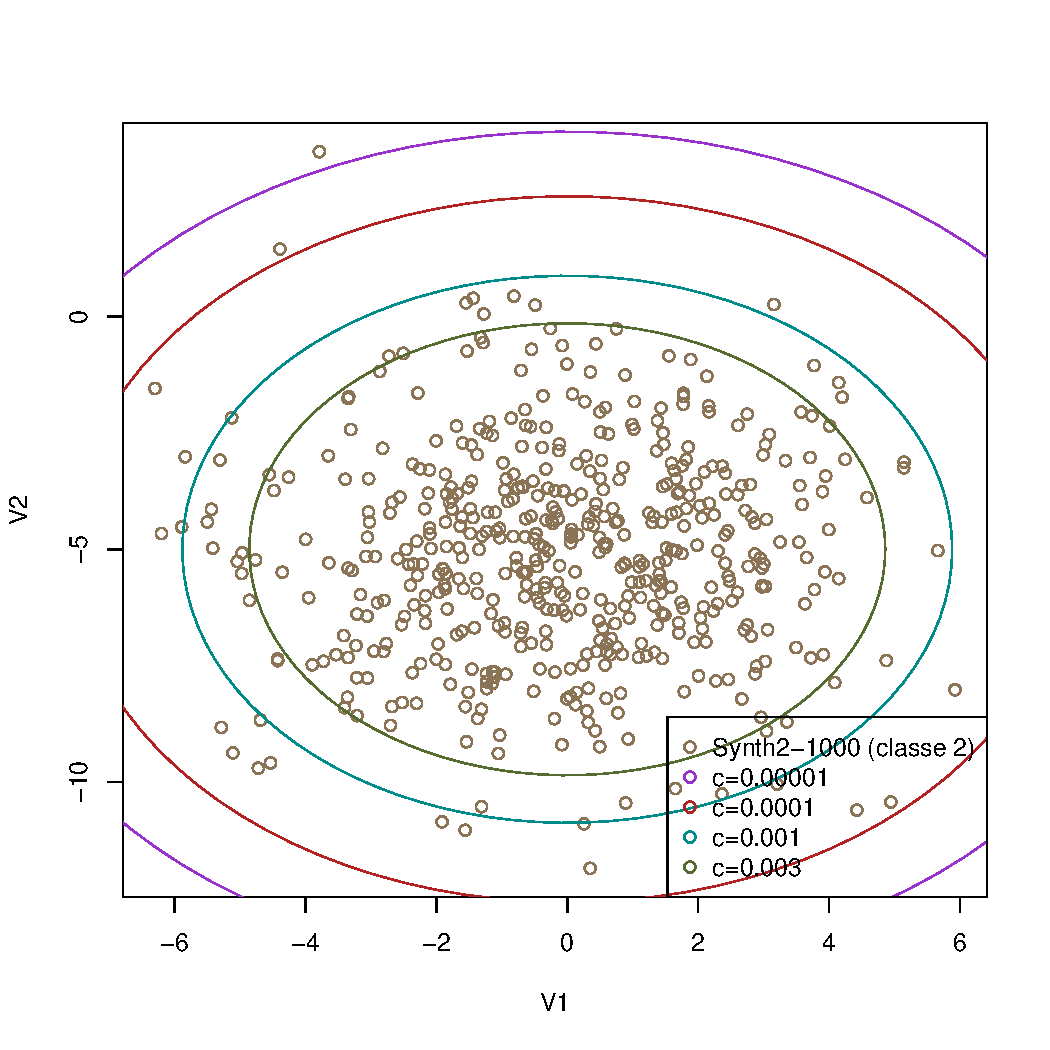
\includegraphics[width=0.35\textwidth]{ellipses.pdf}
    \captionof{figure}{Courbes iso-densité pour $c = 0.003, 0.001, 0.0001, 0.00001$}
    \label{fig_ellipses}
\endgroup

Cherchons maintenant à déterminer l'expression de la règle de Bayes $\delta^{\ast}$ pour le problème de discrimination des classes $\omega_1$ et $\omega_2.$ Sachant que $\delta^{\ast}$ est la règle de décision visant à minimiser la probabilité d'erreur pour un $x$ fixé, cette dernière peut se définir selon l'équation \ref{eq_bayes_rule}.

\begin{equation}
  \label{eq_bayes_rule}
  \delta^{\ast}(x) =
  \left\{
    \begin{array}{rcl}
    	\omega_1 & \text{si} & \mathbb{P}(\omega_2 | x) < \mathbb{P}(\omega_1 | x) \\ 
        \omega_2 & \text{sinon} & \\
    \end{array}
  \right.
\end{equation}

Étant donné que l'on ne travaille qu'avec deux classes, on peut exprimer cette règle en fonction du rapport de vraisemblance. 

Effectivement, 
\[
\delta^{\ast}(x) = \omega_1 \iff 
\mathbb{P}(\omega_2 | x) < \mathbb{P}(\omega_1 | x)
\]

\[
\iff 
\frac{f(x | \omega_2)\pi_2}{f(x)} < \frac{f(x | \omega_1)\pi_1}{f(x)}
\]

\begin{equation}
\label{eq_bayes_rule_max}
\iff 
\frac{\pi_2}{\pi_1} < \frac{f(x|\omega_1)}{f(x|\omega_2)}
\end{equation}

En utilisant l'équation \ref{eq_bayes_rule_max} et en modifiant quelque peu le code source de la fonction \texttt{front.ceuc}, pour les quatre premiers jeux de données, nous avons tracé avec \texttt{R} les frontières de décision dans le plan formé par les variables $X^1$ et $X^2$.

Le résultat obtenu pour le jeu de données présent dans le fichier \texttt{Synth1-1000} est consultable dans la figure \ref{fig_decision_boundary_1000}. Les frontières de décision des jeux de données \texttt{Synth1-40}, \texttt{Synth1-100} et \texttt{Synth1-500} sont consultables en annexe de ce présent rapport (\ref{app_subsec_decision_boundaries})

\begingroup
   \centering
   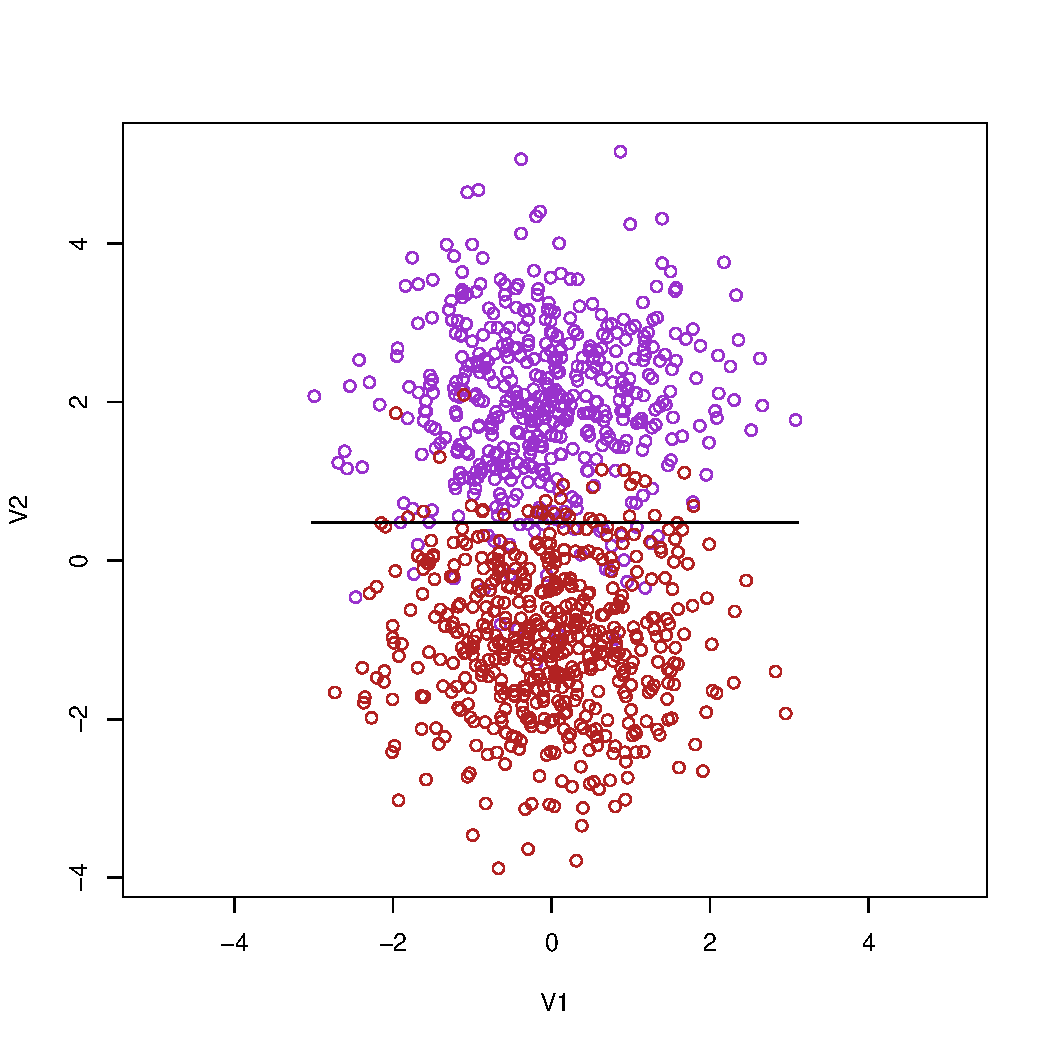
\includegraphics[width=0.35\textwidth]{synth_1_decision_boudary_4.pdf}
    \captionof{figure}{Frontière de décision pour le jeu de données \texttt{Synth1-1000}}
    \label{fig_decision_boundary_1000}
\endgroup


Pour obtenir les résultats dans la figure \ref{fig_decision_boundary_1000}, à l'instar de la fonction \texttt{front.ceuc}, nous calculons le quadrillage d'un "grand" rectangle incluant toutes les données, puis, pour chaque sommet des "petits" rectangles obtenus, nous prenons la décision $\delta^{\ast}$ définie dans l'équation \ref{eq_bayes_rule_max}. En utilisant les sommets entre lesquels $\delta^{\ast}$ change, nous traçons une droite représentant la frontière de décision. 

Sachant que pour les quatre premiers jeux de données, $\Sigma_1 = \Sigma_2 = I_2$ et que $\pi_1 = \pi_2 = 0.5$, nous noterons que la règle de décision précédemment décrite est identique à un simple classifieur euclidien. Effectivement, le calcul de la frontière de décision se ramène à résoudre l'équation \ref{eq_euclidien_classifier}. Le raisonnement pour parvenir à ce résultat est consultable en annexe de ce présent rapport (sous section \ref{app_subsec_bayes_eucl_classifier}).

\begin{equation}
\label{eq_euclidien_classifier}
(\mu_1 - \mu_2)^{T} \left( x - \frac{\mu_1 + \mu_2}{2} \right) = 0
\end{equation}

Ainsi, on pouvait tout simplement se contenter de calculer la médiatrice du segment formé par les deux points $\mu_1$ et $\mu_2$. 

Toutefois, pour l'exercice, nous avons préféré utiliser la méthode qui à nos yeux semblait être la plus complexe. 

Par ailleurs, la première méthode offrait l'avantage non négligeable de nous permettre de tracer la frontière de décision du cinquième jeu de données \texttt{Synth2-1000}. Le résultat obtenu est consultable dans la figure \ref{fig_decision_boundary_2_1000}. On y constate que l'"allure" de la frontière de décision est semblable à celle d'un conique. Or, il s'avère que les frontières de décision des analyses discriminantes quadratiques sont justement des coniques lorsqu'il n'y a que deux classes. A nouveau, cela met en surbrillance la cohérence de nos résultats.   

\begingroup
   \centering
   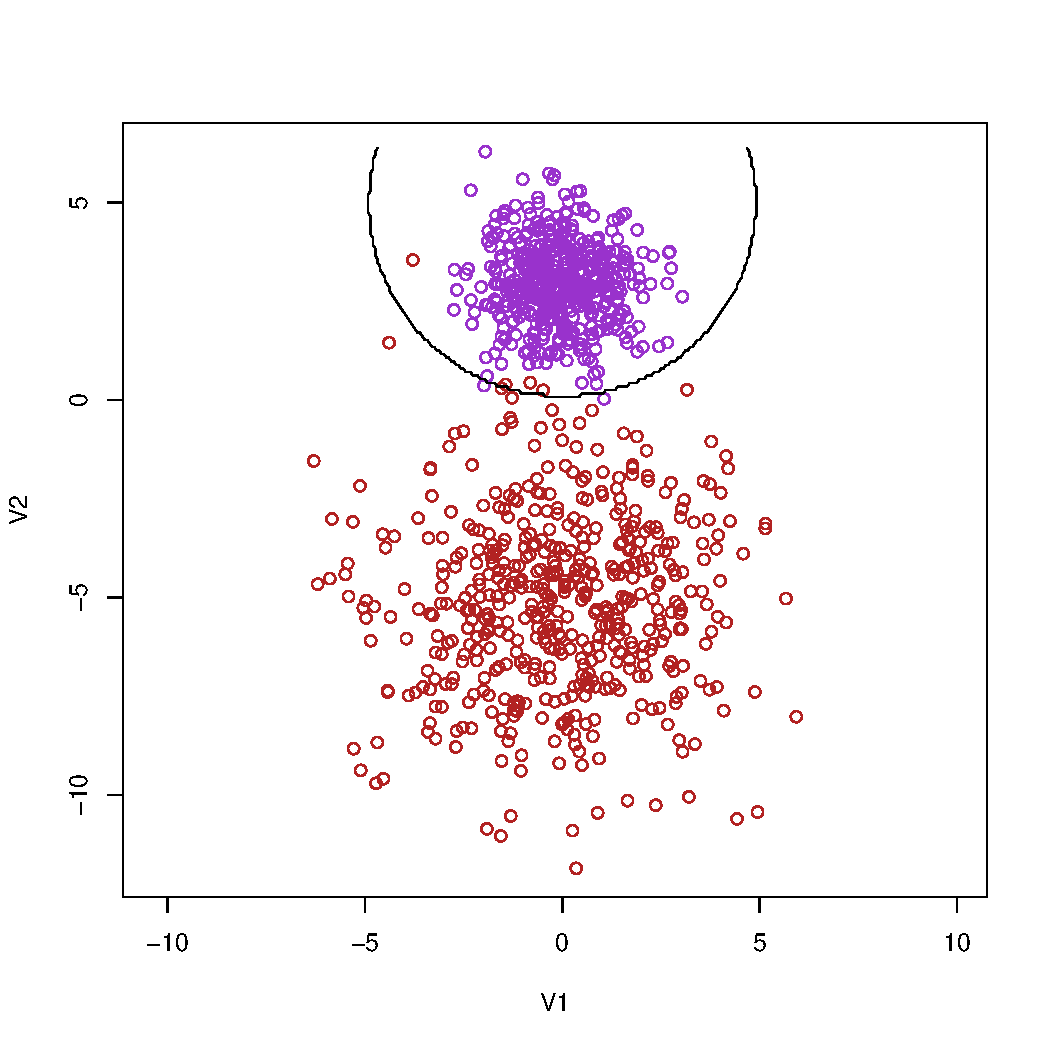
\includegraphics[width=0.35\textwidth]{synth_2_decision_boudary.pdf}
    \captionof{figure}{Frontière de décision pour le jeu de données \texttt{Synth2-1000}}
    \label{fig_decision_boundary_2_1000}
\endgroup

Pour les quatre premiers jeux de données, il était possible de calculer exactement la probabilité d'erreur de Bayes. Les calculs sont grandement simplifiés par le fait que l'on travaille avec $2$ classes et grâce à l'homoscédasticité.

Dans ce cas, la règle de Bayes peut tout simplement s'écrire ainsi :
\begin{equation}
	\label{eq_reecriture_bayes}
  \delta^{\ast}(x) =
  \left\{
    \begin{array}{rcl}
    	\omega_1 & \text{si} & h(x) < \ln(\frac{\pi_1}{\pi_2}) \\ 
        \omega_2 & \text{sinon,} & \\
    \end{array}
  \right.
\end{equation}
où
\[
h(x) = (x -  \frac{\mu_1 - \mu_2}{2})^{T}  \Sigma^{-1} (\mu_2 - \mu_1).
\]
Les éléments pour parvenir à l'équation \ref{eq_reecriture_bayes} sont consultables en annexe de ce présent rapport (sous section \ref{app_reecriture_bayes}).

Après calcul, on peut montrer que, conditionnellement à $\omega_1$,
\begin{equation}
\label{eq_hx_omega_1}
h(X) \sim \mathcal{N}\left( -\frac{\Delta^2}{2}, \Delta^2  \right)
\end{equation}

De plus, on peut montrer que, conditionnellement à $\omega_2$,
\begin{equation}
\label{eq_hx_omega_2}
h(X) \sim \mathcal{N}\left( \frac{\Delta^2}{2}, \Delta^2 \right)
\end{equation}
où $\Delta^2 = (\mu_2 - \mu_1)^T \Sigma^{-1} (\mu_2 - \mu_1)$ le carré de la distance de Mahalanobis entre les deux classes.

On peut alors en déduire la probabilité d'erreur de la règle de Bayes $\epsilon^{\star}$.
\[
\begin{split}
\epsilon^{\star} = \mathbb{P}\left(h(X) < \ln \left(\frac{\pi_1}{\pi_2} \right) | \omega_2 \right) \pi_1 + \\ 
\mathbb{P}\left(h(X) \geq \ln \left(\frac{\pi_1}{\pi_2} \right) | \omega_1 \right) \pi_1
\end{split}
\]

\[
\begin{split}
= \phi \left( \frac{\ln(\frac{\pi_1}{\pi_2}) - \frac{\Delta^2}{2}}{\Delta} \right) \pi_2 + \\ 
\left( 1 - \phi \left( \frac{ \ln(\frac{\pi_1}{\pi_2}) + \frac{\Delta^2}{2}}{\Delta} \right) \right) \pi_1
\end{split}
\]
où $\phi$ représente la fonction de répartition de la loi normale univariée centré réduite.

Pour les quatre premiers jeux de données, étant donné que $\pi = \pi_1 = \pi_2,$ on obtient le résultat suivant :
\[
\epsilon^{\star} = \phi \left( - \frac{\Delta}{2} \right) \pi_2 + 
\left( 1 - \phi \left( \frac{\Delta}{2} \right) \right) \pi_1
\]

\[
\implies \epsilon^{\star} = \phi \left( - \frac{\Delta}{2} \right) (\pi_1 + \pi_2)
\]

\begin{equation}
\label{eq_erreur_bayes_4_jeux_donnees}
\implies  \epsilon^{\star} = \phi \left( - \frac{\Delta}{2} \right)
\end{equation}


Il ne reste alors plus qu'à effectuer l'application numérique de la formule \ref{eq_erreur_bayes_4_jeux_donnees} avec les données à notre disposition. 

\[
\epsilon^{\star} = \frac{1}{\sqrt{2 \pi} } \int_{-\infty}^{ - \frac{\sqrt{(\mu_2 - \mu_1)^T \Sigma^{-1} (\mu_2 - \mu_1)}}{2} } \mathrm{e}^{-\frac 12 t^2} \mathrm{d}t \approx 0.067
\]

Comme prévu, on constate que cette erreur est proche des estimations ponctuelles du taux d'erreur obtenues dans la sous sous section \ref{subsubsec_dataset_1}. De plus, on constate également que $\epsilon^{\star}$ se trouve bien dans les quatre intervalles de confiance calculées dans la même sous sous section. 
\\ \\ \\ \\ \\ \\

\section{Conclusion}
En conclusion, au cours des trois séances de Travaux Pratiques (TP) et de la rédaction du présent rapport, nous avons pu à nouveau prendre conscience de la puissance et des multiples possibilités qui s’offrent à nous en terme de traitement statistique de données avec \texttt{R}. De plus, nous avons pu étudier les performances du classifieur euclidien et des $K$ plus proches voisins sur différents jeux de données binaires. Nous avons également eu l'occasion d'étudier et de mieux comprendre le principe de la règle de Bayes. Enfin, ce TP nous a permis de mieux comprendre ce qu'était l'apprentissage supervisé.

\newpage
\appendix

\section{Code source classificateurs}
\label{app_sec_prog}

\subsection{Classificateur euclidien : ceuc.app et ceuc.val}
\label{app_subsec_prog_ceuc}

\begin{lstlisting}
ceuc.app <- function(Xapp, zapp){
	napp <- dim(Xapp)[1]; # Size of the learning set
	mu1 <- apply( Xapp[which( zapp == 1 ), ], 2, mean ); # Mean of the first class individuals
	mu2 <- apply( Xapp[which( zapp == 2 ), ], 2, mean ); # Mean of the second class individuals
	Mu <- rbind(mu1, mu2);
}

ceuc.val <- function(Mu, Xtst){
	Xtst <- as.matrix(Xtst); # Cast to a matrix
	distXtstMu <- distXY(Xtst, Mu); # Computation of the distances between each individual and each mean
	ptst <- apply(distXtstMu, 1, which.min); # Computation of the index of the nearest mean for each individual
}
\end{lstlisting}

\subsection{$K$ plus proches voisins : kppv.tune et kppv.val}
\label{app_subsec_prog_kppv}

\begin{lstlisting}
kppv.tune <- function(Xapp, zapp, Xval, zval, nppv){
	errorRates <- rep(0, length(nppv)); # It will contain the error rate for each potential K
	i <- 0;
	for(k in nppv){ # Foreach potential k
		i <- i+1;
		pval <- kppv.val(Xapp, zapp, k, Xval);
		errorRates[i] <- errorRate(pval, zval);	
	}
	minErrorRate <- min(errorRates);
	kOptIndex <- max( which( errorRates == minErrorRate ) );
	nppv[kOptIndex];
}

kppv.val <- function(Xapp, zapp, K, Xtst){
	Xtst <- as.matrix(Xtst); # Cast to a matrix
	ntst <- dim(Xtst)[1]; # Size of the test set
	ptst <- rep(1, ntst); # It will contain the predictions
	# Computation of the distances between each individual of the test set
	# and each individual of the learning set	
	distXtstXapp <- distXY(Xtst, Xapp);
	for(i in 1:ntst){ # Foreach individual in the test set
		# We sort the distances between our individual and every individual of the learning set
		sortResult <- sort( distXtstXapp[i, ], index.return = TRUE );
		classes <- zapp[ sortResult$ix[1:K] ] # Classes of the K-nearest neighbours
		tableClasses <- table( factor( classes, levels=c(1, 2) ) ) # To know how much each class is represented
		if(tableClasses[1] >= tableClasses[2]){
			ptst[i] <- 1;
		}else{
			ptst[i] <- 2;
		}
	}
	ptst;
}
\end{lstlisting}

NB : La fonction \texttt{distXY} calcule les distances euclidiennes au carré entre les individus de deux ensembles $X$ et $Y$.

\section{Règle de Bayes}
\label{app_sec_bayes}
Dans les sous sections \ref{app_subsec_bayes_eucl_classifier} et \ref{app_reecriture_bayes}, nous démontrons certaines des formules utilisées dans notre rapport. Ces sous sections nous semblent nécessaires étant donné que ces formules n'ont pas été démontrées dans le polycopié de cours.

\subsection{Frontières de décision pour les jeux de données}
\label{app_subsec_decision_boundaries}

\begingroup
   \centering
   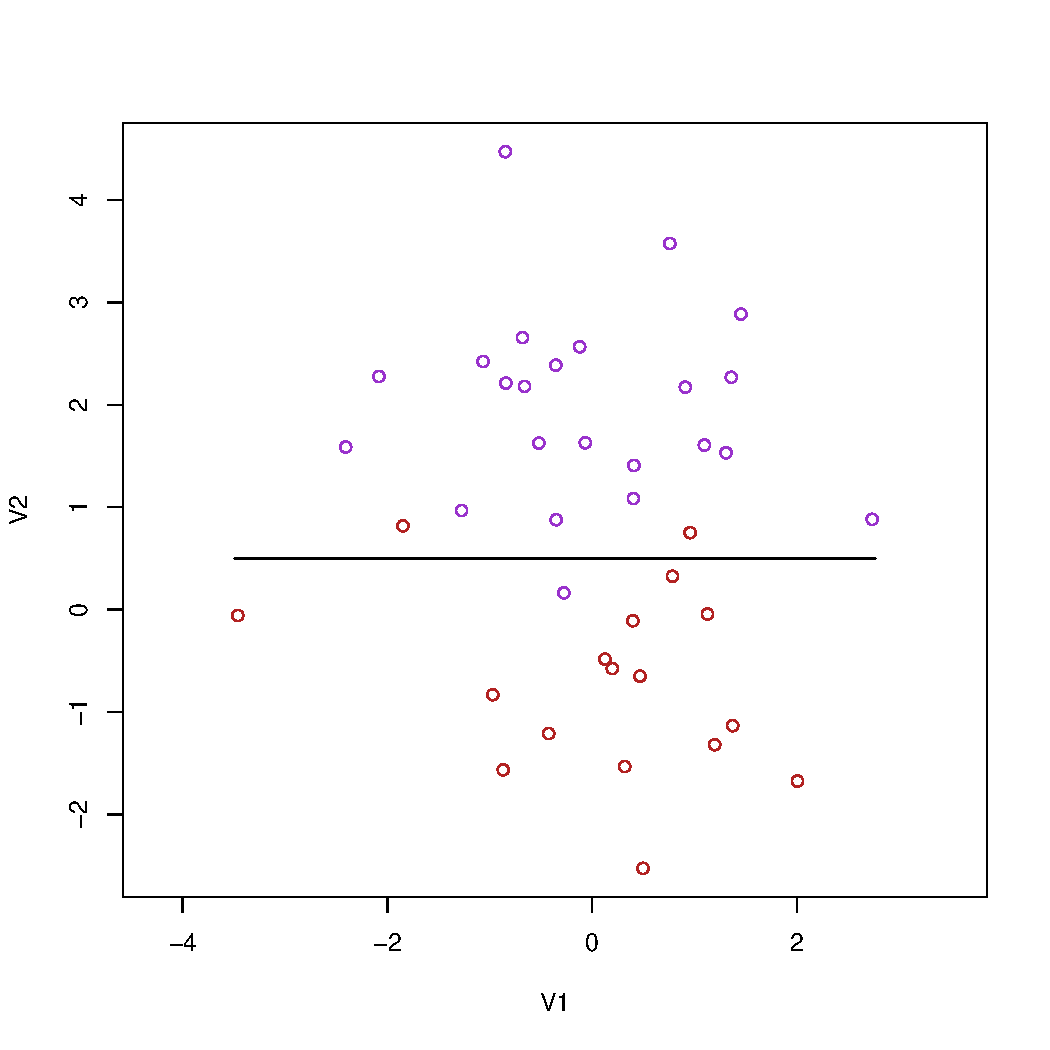
\includegraphics[width=0.35\textwidth]{synth_1_decision_boudary_1.pdf}
    \captionof{figure}{Frontière de décision pour le jeu de données \texttt{Synth1-40}}
    \label{fig_decision_boundary_40}
\endgroup

\begingroup
   \centering
   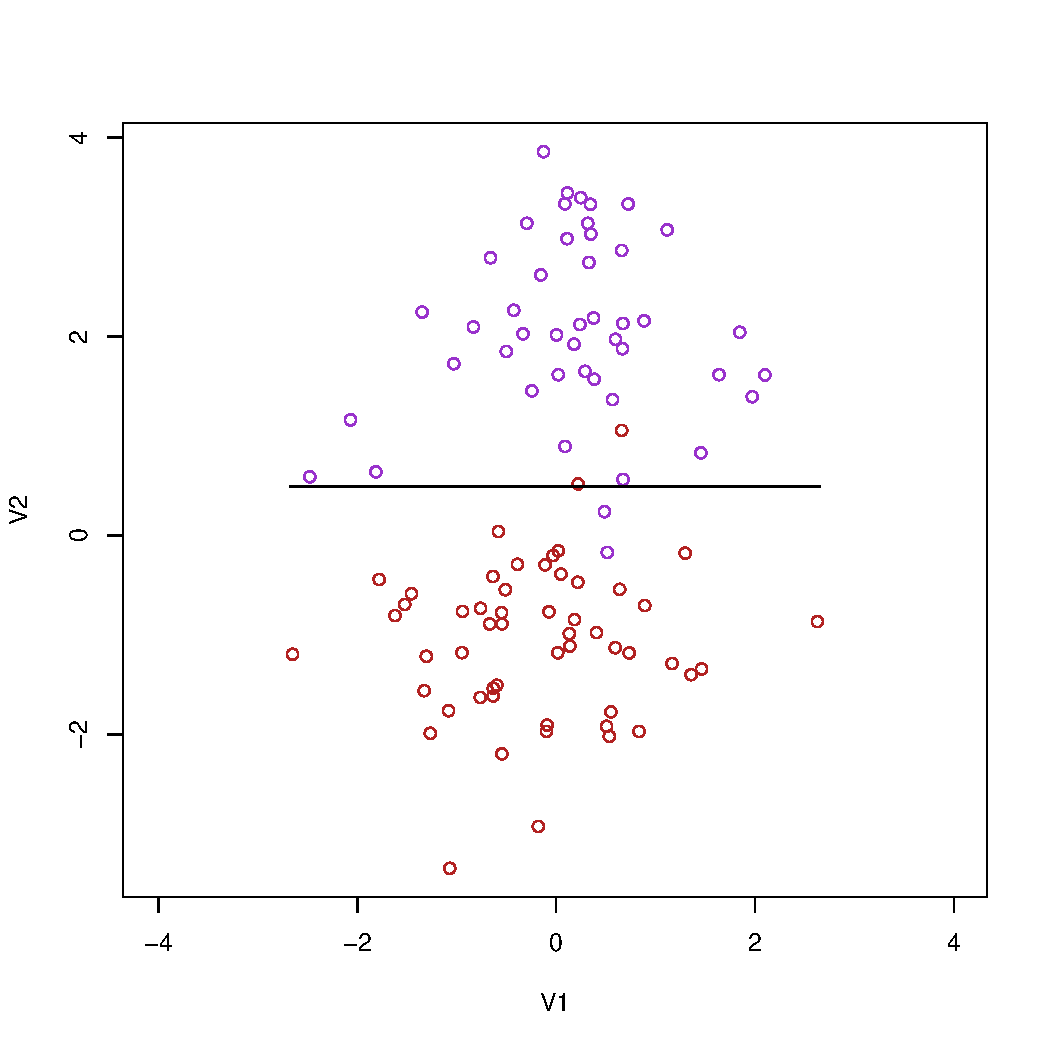
\includegraphics[width=0.35\textwidth]{synth_1_decision_boudary_2.pdf}
    \captionof{figure}{Frontière de décision pour le jeu de données \texttt{Synth1-100}}
    \label{fig_decision_boundary_100}
\endgroup

\begingroup
   \centering
   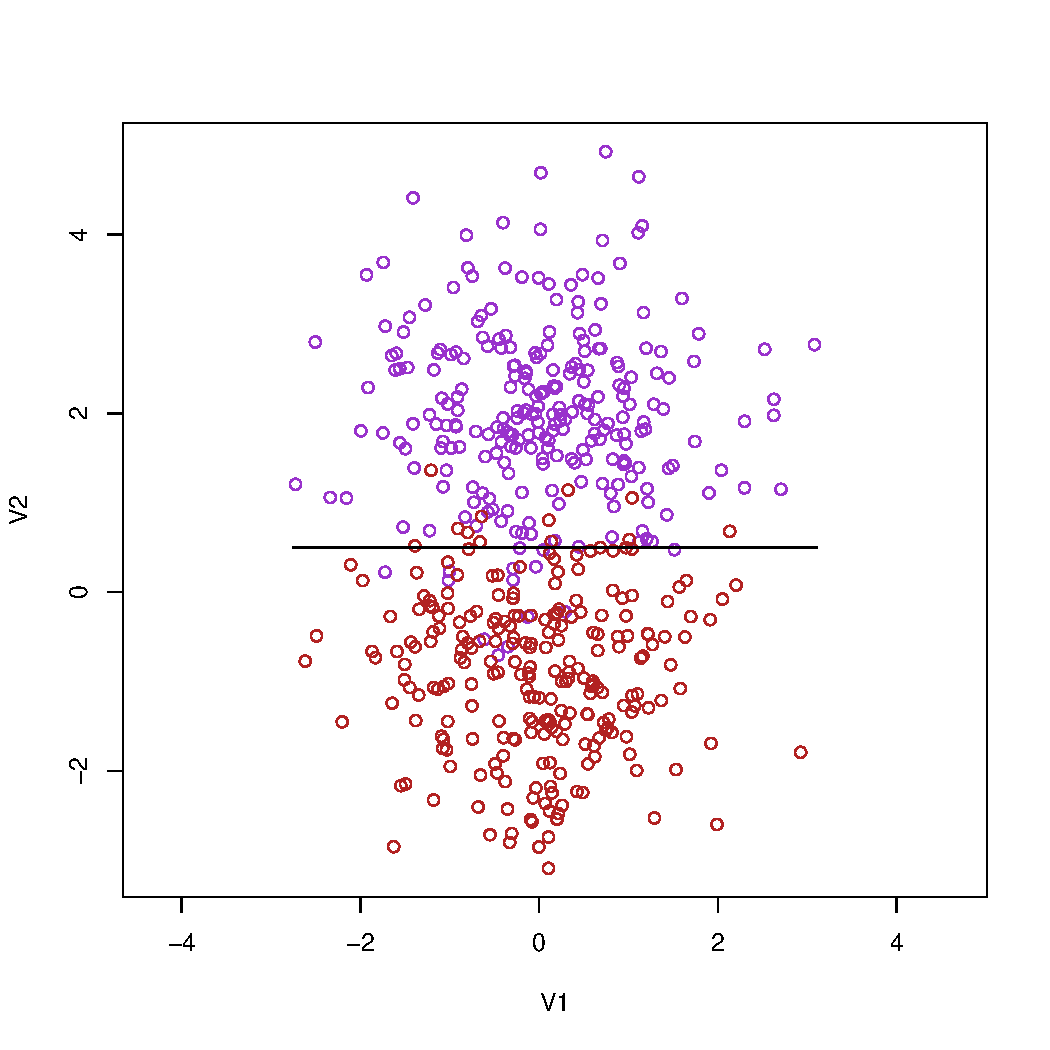
\includegraphics[width=0.35\textwidth]{synth_1_decision_boudary_3.pdf}
    \captionof{figure}{Frontière de décision pour le jeu de données \texttt{Synth1-500}}
    \label{fig_decision_boundary_500}
\endgroup

\subsection{Classifieur euclidien}
\label{app_subsec_bayes_eucl_classifier}
Soit le vecteur forme $X$ suivant, conditionnellement à la classe $\omega_i$, une loi normale bivariée de paramètres $\mu_i$ et $\Sigma_i = I_2 , i \in \{1 ; 2 \}$. On suppose également que les probabilités à priori $\pi_1$ et $\pi_2$ sont égales.

Ainsi,
\[
f(X^1 = x_1, X^2 = x_2 | \omega_i ) = 
\]

\[
= \frac{1}{2 \pi \sqrt{|\Sigma_i|}} \exp \left(-\frac{1}{2}(x - \mu_i)^T \Sigma_i^{-1} (x - \mu_i) \right) 
\]

Or, nous savons que la règle de Bayes $ \delta^{\ast}(x) = \omega_{i^{\ast}},$ où
\[
i^{\ast} =  \operatorname{arg\,max}_i \mathbb{P}(\omega_i | x)
\]

\[
\implies i^{\ast} =  \operatorname{arg\,max}_i \frac{\pi_i f_i(x) }{f(x)}
\]

\[
\implies i^{\ast} =  \operatorname{arg\,max}_i \pi_i f_i(x)
\]

\[
\implies i^{\ast} =  \operatorname{arg\,max}_i \ln(\pi_i f_i(x))
\]

\[
\implies i^{\ast} =  \operatorname{arg\,max}_i \ln(\pi_i) + \ln(f_i(x))
\]

\[
\begin{split}
\implies i^{\ast} =  \operatorname{arg\,max}_i \ln(\pi_i) + \ln \left(\frac{1}{2 \pi \sqrt{|\Sigma_i|}} \right. \\
\left. \exp \left(-\frac{1}{2}(x - \mu_i)^T \Sigma_i^{-1} (x - \mu_i) \right) \right)
\end{split}
\]

\[
\begin{split}
\implies i^{\ast} = \operatorname{arg\,max}_i -\frac{1}{2}(x - \mu_i)^T \Sigma_i^{-1}(x - \mu_i) + \\
\ln(\pi_i) - \ln(2 \pi) - \frac{1}{2} \ln(|\Sigma_i|)
\end{split}
\]

\[
\implies i^{\ast} = \operatorname{arg\,max}_i -\frac{1}{2}(x - \mu_i)^T \Sigma_i^{-1}(x - \mu_i)
\]

\[
\begin{split}
\implies i^{\ast} = \operatorname{arg\,max}_i  -\frac{1}{2}x^T \Sigma_i^{-1} (x - \mu_i) + \\
\frac{1}{2}\mu_i^T \Sigma_i^{-1} (x - \mu_i) 
\end{split}
\]

\[
\begin{split}
\implies i^{\ast} = \operatorname{arg\,max}_i  -\frac{1}{2}x^T \Sigma_i^{-1}x + \frac{1}{2}x^T \Sigma_i^{-1} \mu_i + \\
\frac{1}{2}\mu_i^T \Sigma_i^{-1} x - \frac{1}{2}\mu_i^T \Sigma_i^{-1} \mu_i 
\end{split}
\]

\[
\begin{split}
\implies i^{\ast} = \operatorname{arg\,max}_i \frac{1}{2}x^T \Sigma_i^{-1} \mu_i + \\
\frac{1}{2}\mu_i^T \Sigma_i^{-1} x - \frac{1}{2}\mu_i^T \Sigma_i^{-1} \mu_i 
\end{split}
\]

\[
\begin{split}
\implies i^{\ast} = \operatorname{arg\,max}_i \frac{1}{2}x^T I_2^{-1} \mu_i + \\
\frac{1}{2}\mu_i^T I_2^{-1} x - \frac{1}{2}\mu_i^T I_2^{-1} \mu_i 
\end{split}
\]

\[
\begin{split}
\implies i^{\ast} = \operatorname{arg\,max}_i \frac{1}{2}x^T \mu_i + \\
\frac{1}{2}\mu_i^T x - \frac{1}{2}\mu_i^T \mu_i 
\end{split}
\]

\[
\begin{split}
\implies i^{\ast} = \operatorname{arg\,max}_i \mu_i^T x - \frac{1}{2}\mu_i^T \mu_i 
\end{split}
\]

Posons $g_i(x) = \mu_i^T x - \frac{1}{2}\mu_i^T \mu_i$. La frontière de décision est l'ensemble des solutions $x$ de l'équation \ref{eq_decision_boundary_demonstration}.
\begin{equation}
\label{eq_decision_boundary_demonstration}
g_1(x) = g_2(x)
\end{equation}

\[
\iff \mu_1^T x - \frac{1}{2}\mu_1^T \mu_1 =  \mu_2^T x - \frac{1}{2}\mu_2^T \mu_2
\]

\[
\iff (\mu_1- \mu_2)^T x - \frac{1}{2}\mu_1^T \mu_1 =   - \frac{1}{2}\mu_2^T \mu_2
\]

\[
\iff (\mu_1- \mu_2)^T x - \frac{1}{2}\mu_1^T \mu_1 + \frac{1}{2}\mu_2^T \mu_2 = 0
\]

\[
\begin{split}
\iff (\mu_1- \mu_2)^T x - \frac{1}{2}\mu_1^T \mu_1 + \frac{1}{2}\mu_2^T \mu_2 + \\
\frac{1}{2}\mu_1^T \mu_2 - \frac{1}{2}\mu_1^T \mu_2 = 0
\end{split}
\]

\[
\begin{split}
\iff (\mu_1- \mu_2)^T x - \frac{1}{2}\mu_1^T \mu_1 + \frac{1}{2}\mu_2^T \mu_2 + \\
\frac{1}{2}\mu_2^T \mu_1 - \frac{1}{2}\mu_1^T \mu_2 = 0
\end{split}
\]

\[
\begin{split}
\iff (\mu_1- \mu_2)^T x - \frac{1}{2}\mu_1^T (\mu_1 + \mu_2) + \\
\frac{1}{2}\mu_2^T (\mu_2 + \mu_1) = 0
\end{split}
\]

\[
\iff (\mu_1- \mu_2)^T x + \frac{1}{2} (\mu_2^T - \mu_1^T) (\mu_1 + \mu_2) = 0
\]

\[
\iff (\mu_1- \mu_2)^T x - \frac{1}{2} (\mu_1^T - \mu_2^T ) (\mu_1 + \mu_2) = 0
\]

\[
\iff (\mu_1- \mu_2)^T \left(x - \frac{1}{2}(\mu_1 + \mu_2) \right) = 0
\]

\[
\iff (\mu_1- \mu_2)^T \left(x - \frac{\mu_2 + \mu_2}{2} \right) = 0
\]

\subsection{Réécriture de la règle de Bayes dans le cas avec $2$ classes et avec hypothèse d'homoscédasticité}
\label{app_reecriture_bayes}
Dans cette sous section, nous nous intéressons au cas avec $2$ classes et avec hypothèse d'homoscédasticité ($\Sigma_2 = \Sigma_1 = \Sigma$). Rappelons que la règle de décision de Bayes peut s'écrire ainsi :
\[
\delta^{\ast}(x) = \omega_1 \iff 
\frac{\pi_2}{\pi_1} < \frac{f(x|\omega_1)}{f(x|\omega_2)}
\]

\[
\iff 
\frac{\pi_1}{\pi_2} > \frac{f(x|\omega_2)}{f(x|\omega_1)}
\]

\[
\iff 
\ln \left( \frac{f(x|\omega_2)}{f(x|\omega_1)} \right) < \ln \left(\frac{\pi_1}{\pi_2} \right)
\]

\[
\iff 
\ln ( f(x|\omega_2) ) - \ln ( {f(x|\omega_1)} ) < \ln \left(\frac{\pi_1}{\pi_2} \right)
\]

\[
\begin{split}
\iff 
\ln \left( \frac{1}{2 \pi \sqrt{|\Sigma_2|}} \exp \left(-\frac{1}{2}(x - \mu_2)^T \right. \right. \\
\left. \left. \Sigma_2^{-1} (x - \mu_2) \right)  \right) - \ln \left( \frac{1}{2 \pi \sqrt{|\Sigma_1|}} \right. \\
\left. \exp \left(-\frac{1}{2}(x - \mu_1)^T \Sigma_1^{-1} (x - \mu_1) \right)  \right) < \ln \left(\frac{\pi_1}{\pi_2} \right)
\end{split}
\]

\[
\begin{split}
\iff 
\left(-\frac{1}{2}(x - \mu_2)^T \Sigma^{-1} (x - \mu_2) \right) - \\ 
\left(-\frac{1}{2}(x - \mu_1)^T \Sigma^{-1} (x - \mu_1) \right) < \ln \left(\frac{\pi_1}{\pi_2} \right)
\end{split}
\]

\[
\begin{split}
\iff 
\left(\frac{1}{2} x^T \Sigma^{-1}\mu_2 \right) + \left(\frac{1}{2} \mu_2^T \Sigma^{-1} x \right) + \\
\left(-\frac{1}{2} \mu_2^T \Sigma^{-1} \mu_2 \right) + \left(-\frac{1}{2} x^T \Sigma^{-1} \mu_1 \right) + \\
\left(-\frac{1}{2} \mu_1^T \Sigma^{-1} x \right) + \left(\frac{1}{2} \mu_1^T \Sigma^{-1} \mu_1 \right) \\
< \ln \left(\frac{\pi_1}{\pi_2} \right)
\end{split}
\]

\[
\begin{split}
\iff 
\left(\frac{1}{2} x^T \Sigma^{-1}\mu_2 \right) + \left(\frac{1}{2} x^T \Sigma^{-1} \mu_2 \right) + \\
\left(-\frac{1}{2} \mu_2^T \Sigma^{-1} \mu_2 \right) + \left(-\frac{1}{2} x^T \Sigma^{-1} \mu_1 \right) + \\
\left(-\frac{1}{2} x^T \Sigma^{-1} \mu_1 \right) + \left(\frac{1}{2} \mu_1^T \Sigma^{-1} \mu_1 \right) \\
< \ln \left(\frac{\pi_1}{\pi_2} \right)
\end{split}
\]

\[
\begin{split}
\iff 
\left(x^T \Sigma^{-1}\mu_2 \right) + \left(-x^T \Sigma^{-1} \mu_1 \right) \\
\left(-\frac{1}{2} \mu_2^T \Sigma^{-1} \mu_2 \right) + \left(\frac{1}{2} \mu_1^T \Sigma^{-1} \mu_1 \right) \\
< \ln \left(\frac{\pi_1}{\pi_2} \right)
\end{split}
\]

\[
\begin{split}
\iff 
\left(x^T \Sigma^{-1} ( \mu_2 - \mu_1 ) \right) + \\
\left(-\frac{1}{2} \mu_2^T \Sigma^{-1} \mu_2 \right) + \left(\frac{1}{2} \mu_1^T \Sigma^{-1} \mu_1 \right) \\
< \ln \left(\frac{\pi_1}{\pi_2} \right)
\end{split}
\]

\[
\begin{split}
\iff 
\left(x^T \Sigma^{-1} ( \mu_2 - \mu_1 ) \right) - \\
\frac{1}{2}\mu_2^T \Sigma^{-1} \mu_2 + \frac{1}{2}\mu_1^T \Sigma^{-1} \mu_1 < \ln \left(\frac{\pi_1}{\pi_2} \right)
\end{split}
\]

\[
\begin{split}
\iff \left(x^T \Sigma^{-1} ( \mu_2 - \mu_1 ) \right) - \frac{1}{2}\mu_2^T \Sigma^{-1} \mu_2 + \\ 
\frac{1}{2}\mu_1^T \Sigma^{-1} \mu_1 + \frac{1}{2}\mu_2^T \Sigma^{-1} \mu_1 - \\
\frac{1}{2}\mu_2^T \Sigma^{-1} \mu_1 < \ln \left(\frac{\pi_1}{\pi_2} \right)
\end{split}
\]

\[
\begin{split}
\iff \left(x^T \Sigma^{-1} ( \mu_2 - \mu_1 ) \right) - \frac{1}{2}\mu_2^T \Sigma^{-1} \mu_2 + \\ 
\frac{1}{2}\mu_1^T \Sigma^{-1} \mu_1 + \frac{1}{2}\mu_1^T \Sigma^{-1} \mu_2 - \\
\frac{1}{2}\mu_2^T \Sigma^{-1} \mu_1 < \ln \left(\frac{\pi_1}{\pi_2} \right)
\end{split}
\]

\[
\begin{split}
\iff \left(x^T \Sigma^{-1} ( \mu_2 - \mu_1 ) \right) - \frac{1}{2}\mu_2^T \Sigma^{-1} \\ 
(\mu_2 + \mu_1 ) + \frac{1}{2}\mu_1^T \Sigma^{-1} (\mu_1 + \mu_2) < \ln \left(\frac{\pi_1}{\pi_2} \right)
\end{split}
\]

\[
\begin{split}
\iff \left(x^T \Sigma^{-1} ( \mu_2 - \mu_1 ) \right) + \\
\frac{1}{2} (\mu_1 - \mu_2)^T \Sigma^{-1} (\mu_1 + \mu_2) < \ln \left(\frac{\pi_1}{\pi_2} \right)
\end{split}
\]

\[
\begin{split}
\iff \left(x^T \Sigma^{-1} ( \mu_2 - \mu_1 ) \right) + \\
\frac{1}{2} \left( \Sigma^{-1} (\mu_1 + \mu_2) \right)^T  (\mu_1 - \mu_2)< \ln \left(\frac{\pi_1}{\pi_2} \right)
\end{split}
\]

\[
\begin{split}
\iff \left( x^T \Sigma^{-1} ( \mu_2 - \mu_1 ) \right) + \\
\frac{1}{2} (\mu_1 + \mu_2)^{T} (\Sigma^{-1})^T  (\mu_1 - \mu_2) < \ln \left( \frac{\pi_1}{\pi_2} \right)
\end{split}
\]

\[
\begin{split}
\iff \left(x^T \Sigma^{-1} ( \mu_2 - \mu_1 ) \right) - \\
\frac{1}{2} (\mu_1 + \mu_2)^T (\Sigma^T)^{-1}  (\mu_2 - \mu_1) < \ln \left( \frac{\pi_1}{\pi_2} \right)
\end{split}
\]

\[
\begin{split}
\iff \left(x^T \Sigma^{-1} ( \mu_2 - \mu_1 ) \right) - \\
\frac{1}{2} (\mu_1 + \mu_2)^T \Sigma^{-1}  (\mu_2 - \mu_1) < \ln \left( \frac{\pi_1}{\pi_2} \right)
\end{split}
\]


\[
\begin{split}
\iff \left( x^T - \frac{1}{2} (\mu_1 + \mu_2)^T \right) \Sigma^{-1} \\ 
( \mu_2 - \mu_1 ) < \ln \left( \frac{\pi_1}{\pi_2} \right)
\end{split}
\]

\[
\begin{split}
\iff \left( x^T - \left(\frac{\mu_1 + \mu_2}{2}\right)^T \right) \Sigma^{-1} \\
( \mu_2 - \mu_1 ) < \ln \left( \frac{\pi_1}{\pi_2} \right)
\end{split}
\]

\[
\begin{split}
\iff \left( x - \frac{\mu_1 + \mu_2}{2} \right)^T \Sigma^{-1} ( \mu_2 - \mu_1 ) < \ln \left( \frac{\pi_1}{\pi_2} \right)
\end{split}
\]

\[
\iff
h(x) < \ln(\frac{\pi_1}{\pi_2}),
\]
où
\[
h(x) = (x -  \frac{\mu_1 - \mu_2}{2})^{T}  \Sigma^{-1} (\mu_2 - \mu_1).
\]

\end{multicols}
\end{document}